\chapter{Implementação}

Para validar o conceito apresentado nos capítulos anteriores, a arquitetura do \textit{framework} foi efetivamente implementada e testada.

Neste capítulo serão tratados detalhes de implementação do framework de simulação. Particularidades de implementação e decisões de \textit{design} de software são expostos neste capítulo, assim como alguns exemplos de aplicação e utilização do framework.

Para esta implementação foi utilizada a linguagem \textit{Python}. Toda a comunicação entre máquinas distintas foi feita utilizando \textit{sockets} sobre o protocolo \textit{TCP}. As tarefas assíncronas da implementação foram contruídas sobre a implementação de nativa \textit{threads} provida pela própria linguagem.

\section{A linguagem \emph{Python}}

Python é uma linguagem de programação poderosa e de fácil aprendizado. Possui estruturas de dados de alto nível eficientes, bem como adota uma abordagem simples e efetiva para a programação orientada a objetos. Sua sintaxe elegante e tipagem dinâmica, além de sua natureza interpretada, tornam Python ideal para scripting e para o desenvolvimento rápido de aplicações em diversas áreas e na maioria das plataformas.

O interpretador Python e sua extensa biblioteca padrão estão disponíveis na forma de código fonte ou binário para a maioria das plataformas \cite{PYTHONSITE}, e podem ser distribuídos livremente. Também estão disponíveis distribuições e referências para diversos módulos, programas, ferramentas e documentação adicional, contribuídos por terceiros.

O interpretador Python é facilmente extensível incorporando novas funções e tipos de dados implementados em C ou C++ (ou qualquer outra linguagem acessível a partir de C). Python também se adequa como linguagem de extensão para customizar aplicações.

A linguagem vem sendo amplamnete empregada em desenvolvimento na área de computação científica devido ao seu desempenho satisfatório e sua facilidade de uso. Mais detalhes sobre a linguagem são tratados no apêndice~\ref{appendix_python}.

\section{As camadas externas}

A arquitetura apresentadas nos capítulos anteriores deste documento é representada pelo diagrama \textit{UML} da figura~\ref{fig:arquitetura_uml_geral} (Uma versão expandida, portanto mais completa, deste diagrama pode ser encontrada no anexo~\ref{appendix_uml_completo}). Vale ressaltar que esta representação é completamente independente da linguagem escolhida para sua implementação, porém atrelada ao paradigma de programação orientado à objetos, eleito para construir o \textit{framework} de simulação.

\begin{figure}
  \centerline{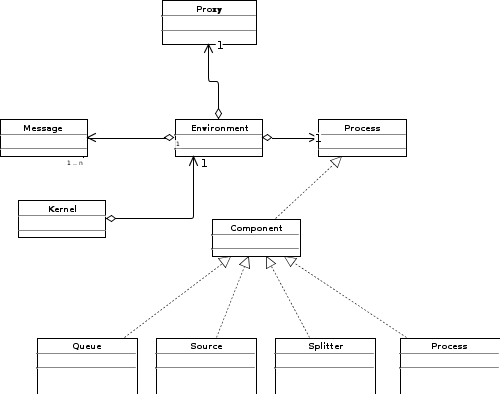
\includegraphics{arquitetura_uml_geral.png}}
  \caption{Diagrama de classes do \textit{framework}.}
\label{fig:arquitetura_uml_geral}
\end{figure}

A arquitetura da árvore de diretórios é ilustrada na listagem~\ref{source_tree}. A partir dela pode-se ilustrar a modularização e a divisão das módulos do framework. Os módulos são descritos a seguir:

\lstinputlisting[language=Python,
                 label=source_tree,
                 caption="Árvore de diretórios do projeto."]{source_tree.txt}

\begin{itemize}
\item \textbf{doc:} Contém toda a documentação do projeto, inclusive esta monografia.
\item \textbf{examples:} Contém exemplos de aplicação do \emph{framework}.
\item \textbf{setup.py:} \emph{Script} de instalação do \textit{framework}.
\item \textbf{t100:} Código fonte do \textit{framework}.
\end{itemize}

Nas seções seguintes são apresentados detalhes internos da estrutura do código implementado. 

\subsection{Módulos internos do \emph{framework}}

O código fonte do \textit{framework} pode ser dividido inicialmente em quatro grandes módulos:

\begin{itemize}
\item \textbf{components:} Possui toda a descrição dos componentes utilizáveis na simulação.
\item \textbf{core:} O módulo \textit{core} possui todos os principais algorítmos internos ao \textit{framework}. São os algorítmos não-modularizáveis do projeto.
\item \textbf{simtool:} O módulo \textit{simtool} possui as implementações de algorítmos modularizáveis do projeto. Neste caso entram algorítmos de sincronismo, de troca de mensagens, etc.
\item \textbf{test:} São os \textit{scripts} de testes do sistemas, necessários para validar a integridade do projeto após eventuais mudanças no código.
\end{itemize}

O módulo \textit{core} possui as especificações mínimas que descrevem componentes e o \textit{kernel} do simulador. São encapsulados também neste nível dados algumas classes de manipulação de erros e algoritmos básicos de execução.

O módulo \textit{components} possui a implementação base necessária para se descrever um componente para a simulação, além de componentes genéricos. Mais detalhes sobre este módulo são tratados na seção~\ref{implement_components}.

\section{Implementando a comunicação}

A linguagem de programação \textit{Python} oferece uma ampla e funcional biblioteca padrão, que provê, de forma nativa na linguagem, métodos para implementação de \textit{threads, sockets}, persistência de dados e estruturas de dados.

Conforme ilustrado na figora~\ref{fig:uml_proxy_basico}, o proxy mínimo de comunicação deve oferecer os seguintes métodos: \textit{send, receive, listen}.

Para a implementação do \textit{proxy} de comunicação 

\section{O objeto \emph{Message}}

Toda a comunicação entre instâncias de \textit{proxy} é realizada enviando e recebendo objetos do tipo \textit{Message}. Um objeto do tipo \textit{Message} é um objeto obrigatoriamente serializável (ou seja, ele pode ser convertido de objeto para um \textit{stream} de bytes a qualquer instante do seu ciclo de vida. Este \textit{stream} de \textit{bytes} deve ser usado para reconstruir o objeto \textit{Message}).

O objeto possuim os campos \textit{content}, que é o conteúdo da mensagem propriamente dito, além dos campos de endereço lógico do remetente e do destinatário. Cabe ao \textit{proxy} converter este endereço lógico em seu correspondente físico antes da transmissão.

\subsection{O método \emph{send}}

O método \textit{send} recebe como parâmetro um objeto do tipo \textit{Message} e o envia para o destinatário designado a ele. O próprio \textit{proxy} deve ser capaz de, em cooperação com o \textit{kernel} do \textit{framework}, resolver o endereço lógico do destinatário para seu correspondendte endereço físico, e realizar a comunicação.


\begin{figure}
  \centerline{\includegraphics{uml_proxy.png}}
  \caption{Diagrama de classes da classe \textit{proxy}.}
\label{fig:uml_proxy_basico}
\end{figure}

\section{Implementando os Componentes \label{implement_components}}
\section{Implementando o \emph{Environment}}
\section{Exemplos de aplicação}

\lstinputlisting[language=Python]{source_prime.py}
